\section{Background \& Related Work}
\label{sec:background}

In this chapter the background information necessary to comprehend Self-Sovereign Identity will be presented. The chapter will start with background concepts to provide some context to the topic, and then it will proceed with what Self-Sovereign Identity is and its core components. Then, related work to this thesis will be presented by means of establishing the state-of-the-art in the area of SSI in the IoT domain.

\subsection{Background Concepts}
\label{subsec:background_concepts}
% [Note: everything leading to SSID goes here]

In this section an overview of the concepts that will be covered during this project will be given in order to provide context and guidance to the rest of this study. At the most introductory level the concept of identity will be grasped, followed by how identities are represented in a digital environment. Afterwards a roadmap will be made on the key architectures for Identity Management Systems on the Internet, where different systems will be covered.

\subsubsection{(Digital) Identity}
\label{subsubsec:digital_identity}

At the time of writing, the way people perceive identity in the real world differs from an actual implementation in the digital world. Before elaborating in this statement, it is best to provide a definition of identity from a philosophical point of view. Looking at Aristotle's Law of Identity, defined in formal logic as "\textbf{A is A -- for any A - Everything is itself}" which can be translated to “each thing is identical with itself” \cite{Telektronikk}. 

Looking at identity from a more recent and practical perspective, provided by the \acrfull{ITU}, identity refers to the representation of an entity in the form of attributes that allow for an entity to be distinguished in a given context \cite{9789261278519}.

On a real-life example, the identity is something originated on a per-relationship basis and that can change over time. The way we present ourselves to someone and the information that recipient gathers is what creates an identity within that relationship. When a person introduces themselves as "Alice" to someone, the other end will process information such as the name, the face, the voice and other relevant attributes to formulate an identity for that specific relation. 
Transporting the concept of identity to the digital world is something that was not envisioned when the internet was created. As a result, an identity layer was missed, leaving users without full control over their identities and leaving the internet designed in a non-user-centric style.

Transporting ITU's definition of identity into the concept of Digital Identity leads to the following definition: "A digital identity is the digital representation of an entity detailed enough to make the individual distinguishable within a digital context" \cite{9789261278519}. A (digital) identity can consist of identifiers (UserID, email, URL, etc.), credentials (certificates, tokens, biometrics, etc.) and attributes (roles, positions, privileges, etc.)\footnote{\url{https://www.itu.int/rec/T-REC-Y.2720-200901-I/en}} and a clear view of how a subject can hold many identities with different identifiers, credentials and attributes can be seen in Figure~\ref{fig:identity_definition}.

\begin{figure}[!ht]
    \centering
    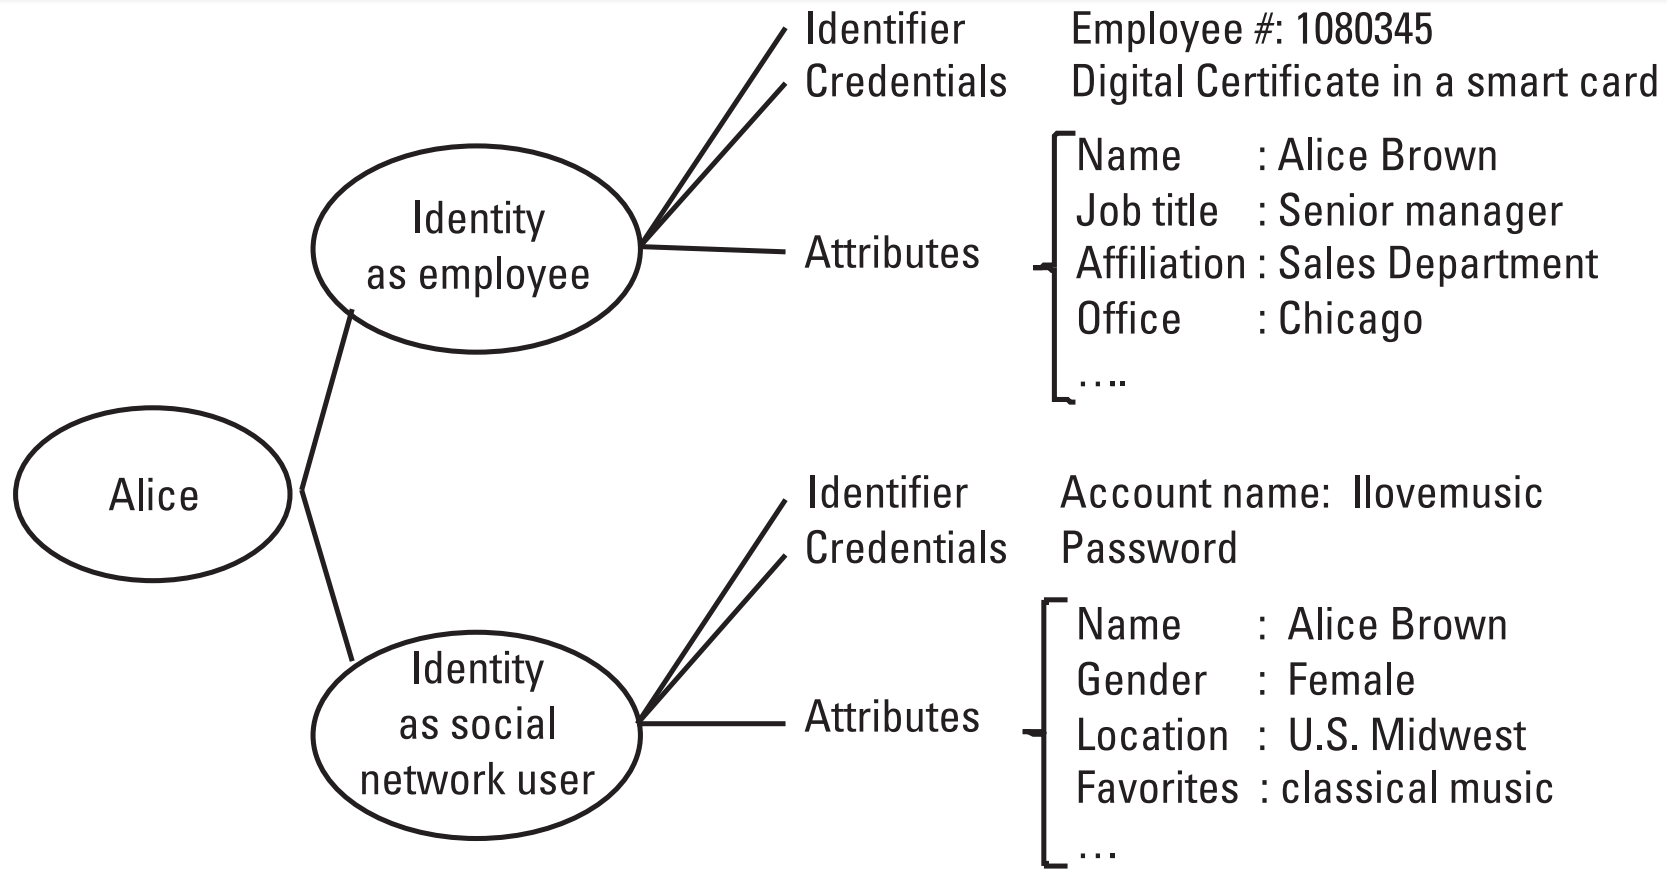
\includegraphics[width=0.8\linewidth]{images/Identity_Definition.png}
    \caption[Structural View on the concept of (Digital) Identity]{Structural View on the concept of (Digital) Identity \cite{bertino2010identity}}
    \label{fig:identity_definition}
\end{figure}

\subsubsection{Identity Management Systems on the Internet}
\label{subsubsec:IdMSs}

Identity Management Systems (IdMSs) are essentially a framework with a predefined set of rules on how digital identities are meant to be commissioned, managed and revoked. In this section light will be shed on the current implementations available to store and manage identities on the Internet, dividing it between two paradigms: Traditional and Decentralized IdMSs.

\paragraph{Traditional IdMSs}

The way Traditional Identity Management Systems were designed was on the basis of three or four actors: Subjects, \glspl{RP}, \glspl{IdP} and in some cases \glspl{CP} \cite{bertino2010identity}. Note that depending on the literature the nomenclature for "Relying Parties" has other definitions such as "Service Provider" \cite{zhu2018identity}. The traditional IdMSs are mainly dependent on a centralized IdP that performs operations of creating, updating, managing and deleting identities of users \cite{gebresilassie2020distributed}. To understand clearly what each party represents, a description extracted from the book by Bertino and Takahashi (2010) \cite{bertino2010identity}, can be found below.
\begin{itemize}
    \item "\textbf{Subjects} are the parties whose identity attributes are digitally recorded and used for transactions and other purposes."
    \item "\textbf{Identity Providers} are the parties that provision identities to subjects."
    \item "\textbf{Relying parties} are the parties that in order to provide services to users (or agents on behalf of users) or access to resources require the submission of proper credentials by users."
    \item "\textbf{Control parties} are typically law enforcement agencies and regulatory bodies that may need access to identity information."
\end{itemize}

The way these parties interact with each other can be summarized using the communication diagram shown in Figure~\ref{fig:interactions_between_different_parties} where it is clear the flow of information between Subjects, RPs and IdPs. Note that since most IdMSs do not require a CP, it has been exempt from this example, but if placed in the diagram it would fall in the center of the triangle and would communicate with all parties as it acts as a regulatory party. The parties depend on each other in the following way: the subject requests access to services from the RP, which in turn requires the IdP to challenge the subject identity through the authentication protocol \cite{zhu2018identity}.

At the dawn of identity management, the solution was truly centralized, since the RPs and the IdPs are combined into one unique entity that acts as the resource server while holding the username and password. This way, traditional identity management models face many challenges including the fact that they rely on a centralized architecture, which in turn leads to single-point-of-failure faults. Also these architectures are more prone to common attacks (e.g. Distributed Denial of Service) given there is a centralized server that can be targeted. Furthermore, in an IoT scenario scalability issues arise, also due to centralization issues. Lastly, and given that most things happen under-the-hood, most systems operate in a non-transparent manner \cite{gebresilassie2020distributed}. This lifts privacy matters, since the users are not fully aware of the practices of an organization, which for example might include their data being sold to 3rd parties.

\begin{figure}[!ht]
    \centering
    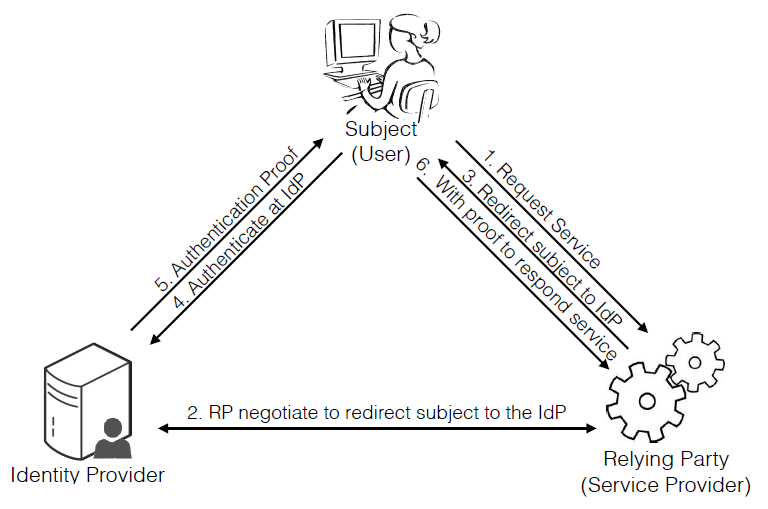
\includegraphics[width=0.6\linewidth]{images/simplified_traditional_IdMS.png}
    \caption[Interactions between different parties in a traditional IdMS]{Interactions between different parties in a traditional IdMS \cite{zhu2018identity}}
    \label{fig:interactions_between_different_parties}
\end{figure}

There is not a single model on how to utilize the Traditional IdMSs. There are four (4) different definitions of models: Isolated, Centralized, Federated and User-Centric. Depending on the systems requirements, a different model is used. However, in general terms, the past IdMSs have evolved from isolated to centralized, and then to federated/user-centric models \cite{JosangAuscertconference}.

\textbf{Isolated Models} are similar to what the web reassembles to today in its majority. Users create different identities for each service they use (mostly usernames and passwords) and they are required to memorize each different identity since the IdP and the SP are combined into one. For example, Facebook creates the identity of the user, but also manages it and manipulates it as they wish (according to regulations).
Since it is up for the users to memorize their identities, and since each service requires different parameters of security (e.g. password must contain 12 characters, 5 numbers and the square root of $\pi$) this can possibly lead to mismanaging identities, password reuse and forgetting credentials \cite{gebresilassie2020distributed}. 

\textbf{Centralized Models} differs from the Isolated Model since it makes use of \acrfull{SSO}, enabling multiple SPs under the same authority to make use of a single IdP. This helps reducing the number of credentials a user needs to memorize, but adds the security liabilities of having a single point of failure, lack of scalability and also introduction to other vulnerabilities and attacks.

\textbf{Federated Models} are similar to Centralized, with the exception that instead of having one authority that controls the Single Sign-On, a consortium of authorities agree with one login that serves for many different services, hence reducing credential management on the user side.

\textbf{User-Centric Models} are more aligned with the need to shift to a paradigm that puts governance in the hands of the users who own the data. This model revolves around users storing the credentials they have in either smart cards or smartphones, but still having the credentials stored in a centralized system provided by the SP. Although it was a step in the right direction it still suffered from the issues causes by relying on a centralized architecture.

\paragraph{Decentralized IdMSs}

With problems such as single point of failure of a centralized IdMS, the privacy concerns that have been reported (Facebook and Equifax data breaches \cite{zhu2018identity} \cite{van2019self} \footnote{\url{https://files.iota.org/comms/IOTA_The_Case_for_a_Unified_Identity.pdf}}), the approach shifted to a decentralized alternative. This approach has in its core the concept of using blockchain, a type of \acrfull{DLT}.

Blockchain was first introduced by Satoshi Nakamoto in the Bitcoin Whitepaper \cite{nakamoto2019bitcoin} and as been defined by the ISO standards as a "distributed ledger with confirmed blocks organized in an append-only, sequential chain using cryptographic links" \cite{ISO22739:2020(en)}. Blockchain consists of a decentralized structure composed of blocks which are linked together in a chronological order. In the Bitcoin implementation proposed by Nakamoto, a Proof-of-Work consensus algorithm is used, this reflects on how the transactions within each block are confirmed and how the blocks themselves get added to the chain. In this consensus mechanism that is allowed by miners who compute highly computational intensive tasks which in turn may return tokens. This latter statement is not the case for all blockchain implementations, but rather it was an example to highlight the usage of blocks and a consensus mechanism.

Blockchains can be of two types: permissioned, when the participants of the network are provided access to it, whereas in a permissionless implementation anyone can enter the network as a new node, which will hold the history of the blockchain, providing a decentralized way for data to be persisted \cite{s18082575} \cite{inbookWang}. 

With DLT it is possible to register every single transaction that gets added to the blockchain. Approaches have been made towards creating such decentralized IdMSs, which include the contributions of big companies such as IBM, and are good starting points for identity to be managed in a more private, secure and distributed way\footnote{\url{http://handle.itu.int/11.1002/1000/11559}}. 

\subsubsection{Paper Credentials Model}
\label{subsubsec:paper_credential_model}

Before diving into Self-Sovereign Identity and understanding how trust can be built around these concepts, it is important to realize how humans have been exchanging information and validating their claims in the past, and still to the time of writing. According to the Oxford Languages dictionary, credential is defined as a "qualification, achievement, quality, or aspect of a person's background, especially when used to indicate their suitability for something"\footnote{\url{https://www.lexico.com/definition/Credential}}. Essentially, a credential can be anything that proves that an individual is eligible for a particular ability (e.g. a driver's license card for driving). These do not need to take the format of a card, but it needs to be something that can bear a certificate that proves it was issued by a trusted party (e.g. the government hologram on the driver's license card). This way, any individual can guarantee that that credential is valid and legitimate. To put it simply, this model handles claims in a trust-based system, since there is no actual infallible method to prove a claim is real.
The basis for this system is composed of three (3) actors: An \textbf{issuer}, a \textbf{holder} and a \textbf{verifier}. Essentially their relationships are summarized in Figure~\ref{fig:paper_credential_model}, where it is clear that the issuer issues a credential to a holder, which when necessary will present it to a verifier. If the verifier trusts the entity which issued the document, it will acknowledge the holders claims as true. 

\begin{figure}[!htb]
    \centering
    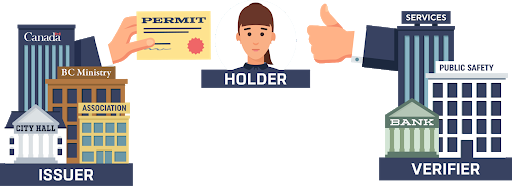
\includegraphics[width=0.7\linewidth]{images/The_Paper_Credential_Model.png}
    \caption[Paper Credential Model]{Paper Credential Model\protect \footnotemark}
    \label{fig:paper_credential_model}
\end{figure}

\footnotetext{\url{https://courses.edx.org/assets/courseware/v1/cb46ed78abdc7583aa95d011426676e0/asset-v1:LinuxFoundationX+LFS172x+3T2019+type\@asset+block/The_Paper_Credential_Model.png}}

At its early beginning (which reports back to the Persian era [Nehemiah 2:1–9]), it was primarily used to allow people with authorization to circulate between lands, provided they could show a document signed by an official authority. Due to the inability to forge documents and create fake copies of an official document, this model worked. But with time, and with the appearance of printers, scanners and software that allows image manipulation, the forging of documents became much easier. That leads to today's age, where the people who need to check for the authenticity of a document (the verifiers) need to be experts in the art of detecting forged credentials.

\subsection{Fundamental Concepts}
\label{subsec:fundamental_concepts}
%[Note: SSID definitely goes here]

In this section the most crucial concepts for this work are presented, with an emphasis on properly introducing the concept and the core enablers of Self-Sovereign Identity. A description of the updated Paper Credentials Model, named Verifiable Credentials Model is given. This is followed by a detailed explanation on the pillars of Self-Sovereign Identity, namely Decentralized Identifiers and the underlying communication protocol DIDComm, Verifiable Credentials and Zero-Knowledge Proofs. The \acrfull{W3C} has been developing specifications that are widely accepted as standards on these topics, and therefore the discussion will be based on these specifications, whose references will be contained in each section.

\subsubsection{Self-Sovereign Identity}
\label{subsubsec:self-sovereign_identity}

\acrfull{SSI} is a key enabler of people being in charge of their own identities. Although it is a field which is still maturing as of the time of writing, it has been coined by Juniper Research as a field which will generate \$1.1 billion in annual revenue by the end of 2024.  \footnote{\url{https://www.juniperresearch.com/press/press-releases/self-sovereign-identity-to-be-a-billion-dollar}}

The term was deeply detailed in an article by Christopher Allen, where he provides a brilliant bridge between the IdMS topic covered before, and the field of SSI:

\begin{quote}
\textit{Self-sovereign identity is the next step beyond user-centric identity and that means it begins at the same place: the user must be central to the administration of identity. That requires not just the interoperability of a user’s identity across multiple locations, with the user’s consent, but also true user control of that digital identity, creating user autonomy. To accomplish this, a self-sovereign identity must be transportable; it can’t be locked down to one site or locale.}\footnote{\url{http://www.lifewithalacrity.com/2016/04/the-path-to-self-soverereign-identity.html}}
\end{quote}

SSI is set to become the next standard for internet communication, as it holds potential to solve many of the internet current trust issues. A brief overview of it can be coined in the following terms: Each entity becomes in charge of its own identity, which means that each user is capable of disclosing only the information and data which they deem relevant or necessary in any relationship they hold. Also, each entity is capable of revoking any piece of data from a relationship or even revoking a relationship entirely, without the need from the other party to consent to this \cite{lo2019analysis} \cite{10.1145/3384943.3409436}. It follows the path of the Decentralized IdMSs that were previously explained, since it utilizes a Distributed Ledger Technology (the blockchain), to enable the usage of \glspl{DID}, \glspl{VC} and enhanced cryptography to support other features such as \glspl{ZKP} \cite{bertino2010identity}. These concepts will be discussed in more detail in the following sections. With the core features mentioned above, SSI disables the need for a central authority to hold any data, and also provides a tamper-proof system that provides transparency and less possibility of forging any credential. Because of the underlying cryptography and blockchain technology, SSI means that an entity can present claims about its identity and others can verify it with cryptographic certainty \cite{liu2020blockchain}. 

\subsubsection{Verifiable Credentials Model}
\label{subsubsec:verifiable_credential_model}

While the Paper Credential Model worked for a long time, due to its many issues with possible forged documents (as documented in Section~\ref{subsubsec:paper_credential_model}), with SSI it is possible to implement the concept of the Verifiable Credentials Model. In 2019 the Verifiable Credential Model has been established as a standard by the W3C \cite{Zundel:19:VCD} \cite{kortesniemi2019improving}.

The foundation for this model is still the same as the Paper Credential Model, there are still 3 parties, namely the Issuer, Holder and Verifier, but a Verifiable Data Registry is added to the picture as a base truth for all the claims that are exchanged in the process.

In order to illustrate each role in this model, the following example will be described making reference to the roles and actions performed by a government, an individual and a vehicle rental agency, in the event of an individual wishing to rent a vehicle. 
The government (issuer) will emit a signed Verifiable Credential (or Claim) to the individual (holder) attesting that they are eligible to drive. The vehicle rental agency (verifier) will request proof that the individual (holder) is eligible to drive. The individual (holder) presents the claim to the vehicle rental agency (verifier), which will check in the Verifiable Data Registry whether the government (issuer) is an entity they trust. Given the claim is cryptographically signed, this prevents it from being a forged document, hence if the vehicle rental agency has the government as a trusted source, the individual has passed the verification process and may rent a vehicle. But, if at some point, the government revokes the individual's credential to be eligible to drive, if the user tries to present the revoked claim to the agency, the agency will know that the user's credential has been revoked. This is the major difference from the paper credential model, since there is no possible way to revoke a physical card which is in the possession of an individual.

A diagram highlighting the flow of interactions in the Verifiable Credentials Model is demonstrated in Figure~\ref{fig:VC_Model}.

\begin{figure}[h]
    \centering
    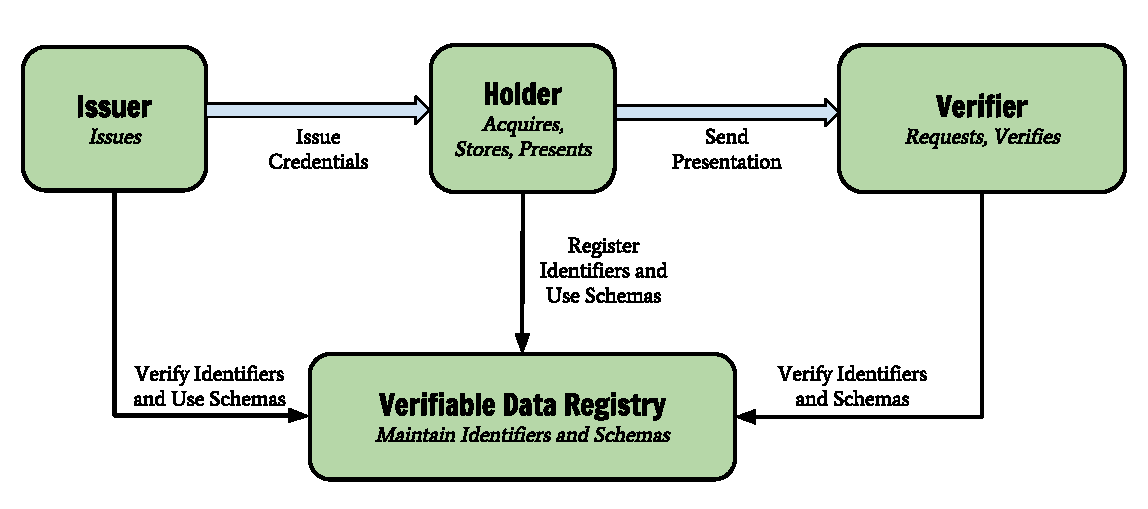
\includegraphics[width=0.7\linewidth]{images/VerifiableCredentialModel.pdf}
    \caption[The Verifiable Credentials Model]{The Verifiable Credentials Model \cite{Zundel:19:VCD}}
    \label{fig:VC_Model}
\end{figure}

\subsubsection{Decentralized Identifiers}
\label{subsubsec:DIDs}

Decentralized Identifiers (DIDs) are the identifiers that power SSI solutions. The aim of this identifier is to provide a scalable way to securely identify each identity that needs to be created. A DID is created for each entity and can be resolved by means of a DID Resolver, which can be seen as the DNS of SSI. Whenever a DID is resolved, it will unveil a DID Document (DIDDoc), which will hold a public key and an endpoint for the other entities to send messages to, allowing them to request for connection establishment  \cite{10.1145/3384943.3409436}. An architectural overview of this process can be found in Figure~\ref{fig:DID_architecture}.
There are two forms of DID, public or pairwise DIDs. While the first is meant to be used by entities that are meant to be "public" and widely contacted (for example a government branch), the latter provides a more secure channel for two entities to connect between each other. The difference between the two in regards to implementation is that Public DIDs are stored in a verifiable public data registry (the blockchain), allowing any entity to have access to this DID. Any individual can request to connect to the entity whose DID is public by creating a connection request. Pairwise DIDs are meant for more secure communication, since for each connection between two different entities, the data for these communications is stored locally, safeguarding from any other entity from eavesdropping, while also reducing the time to start of a connection \cite{terzi2020securing} \cite{theodouli2020towards}.
One of the strongest points with regards to DIDs are that at any time, a DID can be revoked by one of the parties, not allowing for other entities who know this DID to connect to this entity through it. If they wish to do so they must request a new DID for a new relationship to be established \cite{fedrecheski2020self}.

\begin{figure}[t]
    \centering
    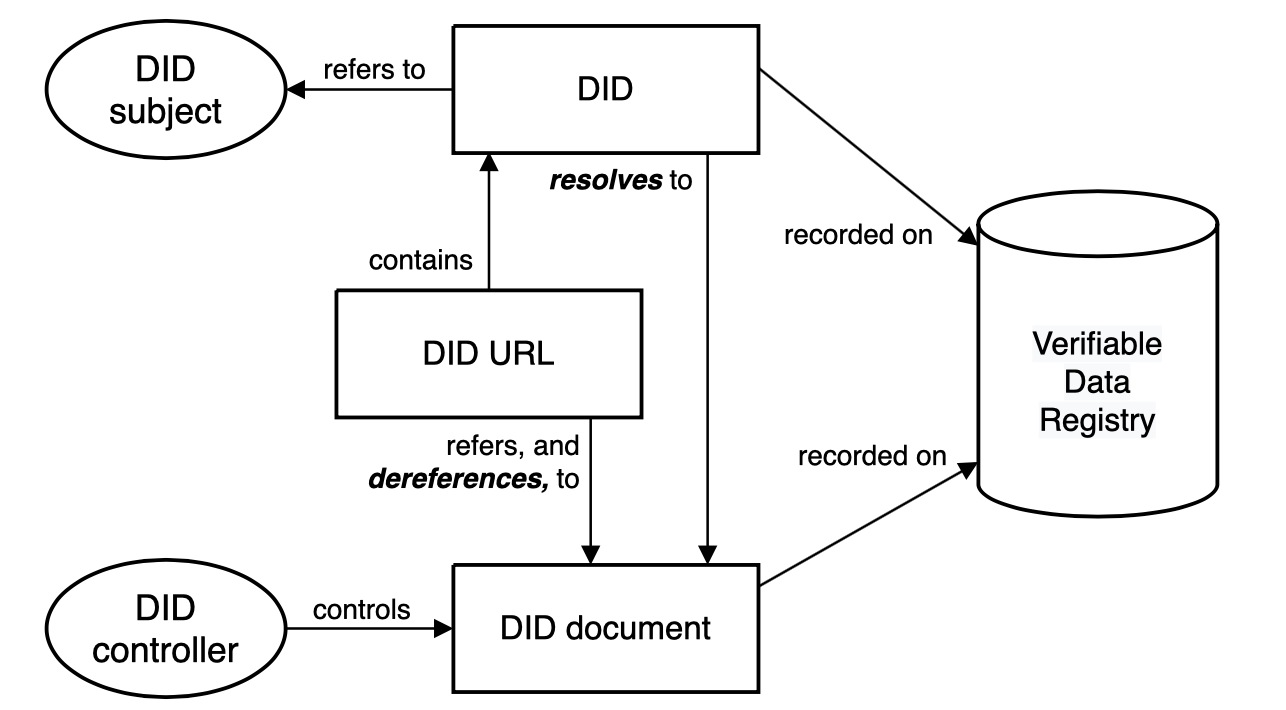
\includegraphics[width=0.6\linewidth]{images/did_brief_architecture_overview.png}
    \caption[Overview of DID architecture]{Overview of the DID architecture \cite{Longley:21:DI}}
    \label{fig:DID_architecture}
\end{figure}

A DID is similar to a universally unique identifier (uuid) for one's identity. Depending on the method used to create the DID, the structure will vary\footnote{\url{https://www.w3.org/TR/did-core/\#did-syntax}}. An example of a DID from the Sovrin network that is going to be discussed further in Section~\ref{subsubsec:hyperledger_indy_sovrin} can be found below:

\begin{verbatim}
    did:sov:AKRMugEbG3ez24K2xnqqrm
\end{verbatim}

The format of the DID follows the standard listed in the official documentation\footnote{\url{https://github.com/WebOfTrustInfo/rwot3-sf/blob/master/did-spec-wd03.md}} and the W3C specification \cite{Sabadello:21:DI}, where it specifies that the substring in between the commas refers to the DID method, which in this case would be of the Sovrin Network DID (\textit{sov}). At the time of writing there are 88 different DID methods listed in the W3C repository\footnote{\url{https://w3c.github.io/did-spec-registries/\#did-methods}}.

\paragraph{Messaging Protocol (DIDComm)}
\label{subsubsec:didcomm}

Although there are many different secure communication mechanisms as detailed in the survey conducted by Nguyen et al. in \cite{nguyen2015survey}, \acrfull{DIDComm}\footnote{\url{https://github.com/hyperledger/aries-rfcs/tree/master/features/0023-did-exchange}} differentiates itself, as it is defined as a protocol whose purpose is to provide a secure, private communication methodology built atop the decentralized design of DIDs\footnote{\url{https://identity.foundation/didcomm-messaging/spec/}}.

The methodology of DIDComm is based on the usage of the information that is present in the DID Documents to allow for secure,
private, decentralized, transport-agnostic, routable, interoperable, extensible, efficient communication between two individuals through their agents \cite{SovrinIotSSI}. 

The messaging format of DIDComm as defined by W3C uses JSON Web Messages\footnote{\url{https://identity.foundation/didcomm-messaging/spec/\#:~:text=DIDComm\%20plaintext\%20messages\%20are\%20based,message\%2C\%20and\%20are\%20called\%20headers.}}, and depending on the action to perform (issue credentials, request for a credential presentation, etc), the fields will vary. An example of a "Basic Message" structure would contain the following fields:

\begin{verbatim}
{   
    "id": "1234567890",
    "type": "<message-type-uri>",
    "from": "did:example:alice",
    "to": ["did:example:bob"],
    "created_time": 1516269022,
    "expires_time": 1516385931,
    "body": {"messagespecificattribute": "and its value"}
}
\end{verbatim}

\subsubsection{Verifiable Credentials}
\label{subsubsec:VCs}

Verifiable Credentials or Claims (VCs) are the pieces of technology in the digital world that mimic the physical credentials people bear with them on a regular basis like their passport, bank account number, amongst others. Verifiable Credentials are powered by digital signatures (powered by cryptography) making them verifiable and tamper-proof. The format of the VCs follows the standard listed by the W3C specification \cite{Sabadello:21:VCs}.

The way VCs can be adopted into people's lifes is by following the Verifiable Credentials Model previously mentioned in Section~\ref{subsubsec:verifiable_credential_model}. An example of how the fields (attributes) within the standard paper credentials can be ported to a Verifiable Credential is demonstrated in Figure~\ref{fig:example_VC}, where the Issuer Signature is missing since it refers to (in the example) the California Department of Motor Vehicles.
\begin{figure}[!htb]
    \centering
    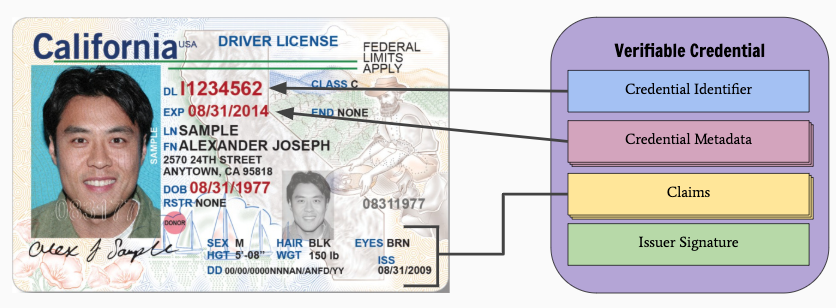
\includegraphics[width=0.7\linewidth]{images/Verifiable_Credentials.png}
    \caption[Example of how attributes from a paper crendential can be stored in a Verifiable Credential]{Example of how attributes from a paper crendential can be stored in a Verifiable Credential \protect\footnotemark}
    \label{fig:example_VC}
\end{figure}
In order to issue a credential, an issuer needs to use a credential schema that is present on the ledger, containing details on which information composes a credential under that schema.
\footnotetext{\url{https://freecontent.manning.com/the-basic-building-blocks-of-ssi}}
Whenever an issuer creates a schema, the ledger will create a response containing an identifier for that particular schema. If an issuer wishes to start issuing credentials under the schema listed above, they need to submit a credential definition onto the ledger mentioning the ID of the schema (provided earlier) and other fields like type of signature method, how to handle revocation and so on.\footnote{\url{https://hyperledger-indy.readthedocs.io/projects/sdk/en/latest/docs/how-tos/save-schema-and-cred-def/README.html}}

Figure~\ref{fig:relation_between_credential_schema_and_definition} holds an example of the link between a credential schema (which in the example is issued by the government), and the credential definition (who is created by an entity named "Faber"). Here is it possible to see how the credential definition contains the information regarding the schema as one of its fields. 

\begin{figure}[!htb]
    \centering
    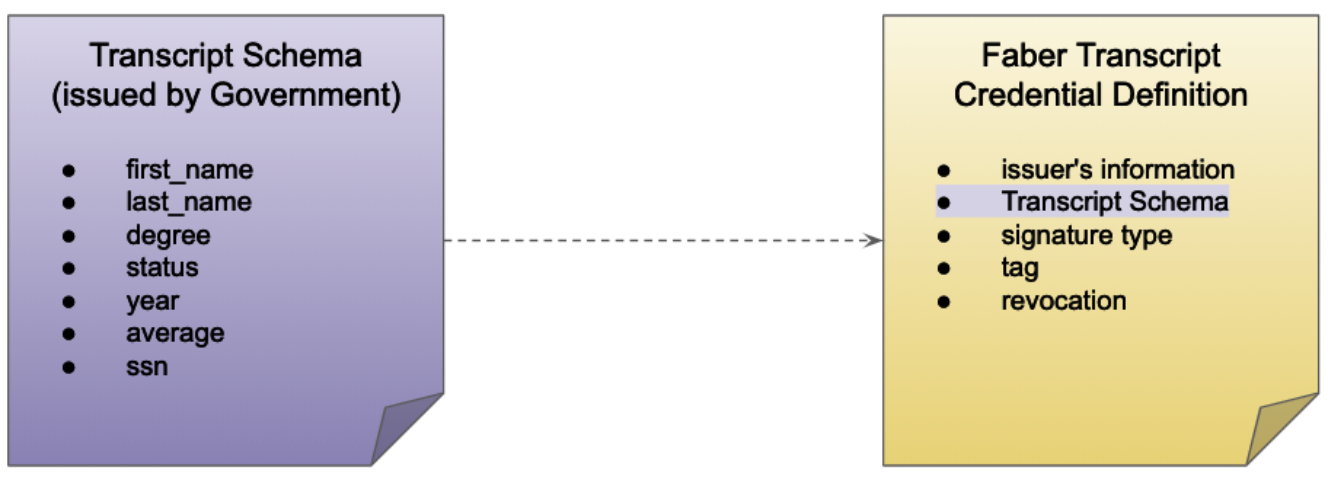
\includegraphics[width=0.7\linewidth]{images/schema-credential.png}
    \caption[Relation between credential schema and credential definition]{Relation between credential schema and credential definition \protect\footnotemark}
    \label{fig:relation_between_credential_schema_and_definition}
\end{figure}

\footnotetext{\url{https://kctheservant.medium.com/exploring-hyperledger-indy-through-indy-dev-example-10075d2547ae}}

Below an example of a credential object is presented, in the JSON Web Message format, containing the attributes, the credential\_definition\_id, revocation\_id and schema\_id.

\begin{verbatim}
    {
      "attrs": {
        "additionalProp1": "string",
        "additionalProp2": "string",
        "additionalProp3": "string"
      },
      "cred_def_id": "WgWxqztrNooG92RXvxSTWv:3:CL:20:tag",
      "cred_rev_id": "12345",
      "referent": "3fa85f64-5717-4562-b3fc-2c963f66afa6",
      "rev_reg_id": "WgWxqztrNooG92RXvxSTWv:4:WgWxqztrNooG92RXvxSTWv:3:CL:20:tag:CL_ACCUM:0",
      "schema_id": "WgWxqztrNooG92RXvxSTWv:2:schema_name:1.0"
    }
\end{verbatim}

\subsubsection{Zero-Knowledge Proof}
\label{subsubsec:ZKP}

The concepts of Zero-Knowledge Proofs is its majority powered by advancements in Mathematics and Cryptography and are one of the best ways to preserve individuals identities whenever they need to present any claim about themselves.
The moving force behind ZKP is the fact that an individual must not need to disclose any of its attributes in order to validate a claim. The Verifiable Credentials Model has already linked the implementation of ZKPs together with VCs in order to enable data minimization and privacy enhancement, as provers can present proof with minimal disclosure of sensitive and personal data to the verifiers \cite{terzi2020securing}\cite{Zundel:19:VCD}. To enhance privacy and security furthermore, the claims presented by the VC can take the form of a predicate ZKP or selective disclosure ZKP. 

\paragraph{Predicates in ZKP}

Predicates are used in ZKP whenever a holder needs to attest that he/she is in compliance with a requirement linked to one of its attributes without disclosing the data linked to that attribute \cite{bertino2010identity} \cite{bartolomeu2019self}. 
One of the predicates which is supported by VCs is the greater or equal to ($>=$). Using this predicate and formulating a real-life scenario would be for when an individual wants to demonstrate that he is over the age of 18 in order to request any alcoholic drink at a bar. Usually this process requires handing in the personal ID, in order for the barman to analyze the date of birth and calculate whether the individual is over the age of 18. With predicates in ZKP, the verifier (barman) would request proof that the individual (holder) is over the age of 18, which in turn would craft a Verifiable Presentation using ZKP, which can (by cryptographic means) validate that the user is older than 18, without ever disclosing the date of birth of the individual.

\paragraph{Selective Disclosure in ZKP}

Still picking up on the example of the individual who is required to demonstrate he is over the age of 18, despite that being a very ineffective process, it also discloses other information to the barman which are not relevant to that transaction. The ID is a Credential composed of many attributes which have relevance depending on the scenario. Hence, in a Verifiable Credentials Model using Selective Disclosure in ZKPs, a user can craft a presentation to show to the barman only the relevant piece of information (attributes) from a Verifiable Credential \cite{fedrecheski2020self}. This way the individual chooses to only disclose the date of birth from its ID in the form of a VC, and shows that newly crafted VC to the barman, without ever needing to disclose other pieces of data commonly found in a paper ID \cite{davie2019trust}. 

\subsubsection{Revocation of VCs}
\label{subsubsection:revocation_registries}

An issuer may want to revoke credentials, for the same reasons why paper credentials are revoked in the Paper Credentials Model: either they expire, or the holder lost privilege to hold them. Using the already mentioned driver's license example, if the driver loses too many points, the driver will be stripped off their driver's license so that they cannot drive anymore. With VCs, this event could be handled by revoking the credential that attests as the driver's license of the driver. In order to revoke a credential, the issuer of said credential writes a revocation registry and adds it to the Verifiable Data Registry. When revoked, the credential is no longer valid, and any verifier will be aware of this revocation by looking into the Verifiable Data Registry and being presented with the revocation registry of that credential.
The revocation registry links back to the credential, and allows the issuer to unilaterally revoke credentials, independently of the holders. Depending on the adopted DLT, the implementation for the revocation registry might differ\footnote{\url{https://tykn.tech/identity-revocation-blockchain/\#What_is_a_Revocation_Registry}}.

\subsubsection{Management of DIDs and VCs}
\label{subsubsec:wallets_and_agents}

An important aspect that was not yet discussed is how DIDs and VCs are handled and where they are stored. For this end, digital identity wallets, which are pieces of software purposefully created to store DIDs and VCs were envisioned\footnote{\url{https://freecontent.manning.com/the-basic-building-blocks-of-ssi/\#id_ftn4}}. On the other hand, in order to be part of the Verifiable Data Model and interact with other entities, there needs to be a piece of software that allows to manage and use the VCs that the entities hold in their wallets. That is the role of an agent, which can be defined as a software used by or acting on behalf of an entity to interact with other agents. Agents require access to a digital wallet in order to perform cryptographic operations on behalf of the entity that they represent\footnote{\url{https://sovrin.org/library/glossary/}}. 

Agents are in charge of sending and receiving messages; encrypting and decrypting information; sign digital information on behalf of the entity; manage information in the digital wallet and backup/restore information \cite{SovrinIotSSI}. The SSI community has advocated that an agent can also be referred to as a wallet, since most agents offer an integrated wallet as one of its components \footnote{\url{https://iiw.idcommons.net/Agent/Wallet\%3F_What_is_Agent\%3F_What_is_Wallet\%3F_Are_They_The_Same\%3F}}. This makes the two terms interchangeable in the literature.

Some agents contain the implementation to interact with the Verifiable Data Registry (i.e. Distributed Ledger), to allow for the adoption of the Verifiable Data Model. They can be of three different types: 

\begin{itemize}
    \item Edge agents run at the edge of the network on a local device;
    \item Cloud agents run remotely on a server or cloud hosting service
    \item Mobile agents are meant to be hosted on the entities' private device (e.g. smartphones)
\end{itemize}

The biggest difference worth denoting in the different types of agents is that cloud agents provide a public endpoint for interactions with other agents, with this endpoint being publicly available in the Verifiable Data Registry. Therefore, a person whose privacy is more important might be better using a mobile agent on their device, while an organization might have an agent running on the cloud. For IoT devices for example, it would be interesting to consider an edge agent as the preferred agent type. For the latter, lacking compute/storage resources and/or connectivity, securely communicating with a cloud agent that in turn communicates with the ledger \footnote{\url{https://github.com/hyperledger/aries-cloudagent-python/blob/main/docs/GettingStartedAriesDev/AriesBigPicture.md}} would be a possible alternative to the fact that these agents have no public endpoint.

\subsubsection{Relation with Distributed Ledger Technology}
\label{subsec:what_information_goes_onto_the_DLT?}

After covering DIDs and VCs, it is important to understand what gets stored on the Distributed Ledger. The most relevant note to be made is that no private data is stored on the blockchain, which provides any solution using a DLT with an increased privacy-preserving solution. The blockchain will only hold the Public DIDs, the Schemas, the Credential Definitions and the Revocation Registries. 

\subsection{Blockchain-based Self-Sovereign Identity with IoT}
\label{subsubsec:Blockchain-based_SSI_with_IoT}
%[Note: related work goes here]

In this section the related work will be discussed in detail, looking at the state-of-the-art research that has been put together with the aim of exploring Self-Sovereign Identity's integration into IoT environments.

For this purpose, the results from the numerous search queries are illustrated in Table~\ref{tab:related_work}. Note that for IEEEExplore and ACM (Digital Library), since these were extracted after Google Scholar, many of the papers listed under Google Scholar were also found repeated under the other two sources. The search terms utilized are listed in Table~\ref{tab:related_work_queries}.

\begin{table}[!ht]
    \centering
    \begin{threeparttable}[h]
        \begin{tabular}{|l|c|c|c|c|}
        \hline
            \backslashbox{Topic}{Source} & Google Scholar & IEEEExplore & DL & Other\tnote{1}\\
             \hline
            SSI + IoT & \cite{terzi2020securing}, \cite{gebresilassie2020distributed}, \cite{fedrecheski2020self}, \cite{bartolomeu2019self}, \cite{kulabukhova2019self} & \cite{theodouli2020towards} & \cite{10.1145/3352411.3352435} & \cite{kortesniemi2019improving}\\
            \hline
            SSI & \cite{van2019self} & \sout{ } & \sout{ } & \sout{ }\\
            \hline
            IdMSs for IoT & \cite{luecking2020decentralized}, \cite{zhu2018identity}, \cite{lo2019analysis}, \cite{10.1145/3384943.3409436}, \cite{liu2020blockchain},  \cite{zhu2017autonomic} & \sout{ } & \sout{ } & \sout{ }\\
            \hline
            SSI + Energy & \cite{cheddadi2020design}, \cite{dekker2020automating}, \cite{wang2019energy} & \sout{ } & \sout{ } & \sout{ }\\
            \hline
        \end{tabular}
        \begin{tablenotes}
        \item[1] Supervisor Literature, Back- and For-ward referencing.
        \end{tablenotes}
    \end{threeparttable}
    \caption{Summary of Literature}
    \label{tab:related_work}
\end{table}

\begin{table}[!ht]
    \centering
    \begin{threeparttable}[h]
        \centering
        \begin{tabular}{|p{0.2\linewidth}|p{0.7\linewidth}|}
        \hline
            \multicolumn{1}{|c|}{\textbf{Repository}} & \multicolumn{1}{c|}{\textbf{Search Terms}}\\
            \hline
            Google Scholar & "Self Sovereign Identity" \& "+"Self+Sovereign+Identity" +"Internet+of+Things" \& "Decentralized Identifiers"\\
            \hline
            IEEEExplore & "Self Sovereign Identity with IoT Blockchain" \\
            \hline
            ACM & "Self Sovereign Identity Internet of Things Blockchain" \\
            \hline
        \end{tabular}
        \begin{tablenotes}
        \end{tablenotes}
    \end{threeparttable}
    \caption{Literature Search Terms}
    \label{tab:related_work_queries}
\end{table}

\subsubsection{Blockchain as an IdMS}
\label{subsubsec:blockchain_as_an_IdMs}

The adoption of blockchain as a Decentralized IdMS has been widely acclaimed as a good alternative to handle access control as an alternative to the previous alternatives, namely ABAC (Attribute-based access control) and
RBAC (Role-Based Access Control), since it has been proved that these are inflexible, unscalable and difficult to upgrade \cite{liu2012authentication}. Despite blockchain-based IdMSs being coined the best alternative to traditional IdMSs \cite{10.1145/3352411.3352435}, these systems still present other issues compared to conventional IdMSs. Issues such as how to handle digital wallet leakage; identity changes; the underlying infrastructure and the key management of the public and private keys are some of the matters which need to be overcome in order to solidify blockchain as a definite substitute for traditional IdMSs \cite{liu2020blockchain}. 

\paragraph{Blockchain IdMS for IoT}

In a paper by Salah \cite{inproceedingsSalah} an analysis was made on different IoT access control approaches and the novel architecture based on blockchain proved to outperform OAuth2, OAuth0, Manual Device Authentication and Blockstack in the selected quality attributes (availability, scalability, decentralization and tamper-Proofness).

Being a distributed, incorruptible and tamper-resistant ledger database, blockchain has the potential to address the critical security issues of IoT, particularly on data integrity and reliability \cite{inbookWang}. 

However, not all types of blockchain are capable of serving IoT devices' needs. This is the case for permissionless blockchains, as they usually utilize proof-of-work consensus algorithms that are computationally expensive and involve high bandwidth overheads and delays. This in turn restricts the number of transactions per second that can occur \cite{luecking2020decentralized} \cite{lupascu2020dlt}. Hence, the best alternative is to utilize a permissioned blockchain for a possible IoT IdMS \cite{lo2019analysis}. 

The main challenges which need to be overcome in order to provide a standardized solution for IoT blockchain-based IdMSs are: computational power, energy demand and storage capabilities of IoT devices, mobility and partition of said devices and lastly the latency and capacity of communication to and from devices \cite{inbookWang}. On a survey conducted by Lo et al. \cite{lo2019analysis} more issues have been gathered regarding IoT devices and how these can affect a possible IdMS. Again, matters of resource consumption are identified with a scope on how encryption is made on the sensor data. Single point of failure, lack of standardization on managing IoT devices and interoperability are also matters related to IoT identified by this survey.

Matters of confidentiality, privacy and data integrity are also concerns in an IoT environment, and blockchain presents itself as a candidate for solving these issues. Blockchain grants authenticity, non-repudiation, and integrity by default, and if smart contracts are used to manage authorization and automate transactions, this satisfies the need for confidentiality, privacy and data integrity \cite{s18082575}. Despite the good prospects of blockchain, it still contains some drawbacks, such as ensuring security of computation, since the computational capability of blockchain is still limited; and also, due to the latency caused by some consensus algorithms on public blockchains, a system running with blockchain cannot support real-time monitoring \cite{lo2019analysis}.

The existing solutions for IoT blockchain-based IdMSs mostly represent generic solutions. However the domain-specific solutions regard the manufacturing domain, automotive, electric trading, energy grid, eHealth and smart home, according conducted surveys on the matter \cite{lo2019analysis}. One of the earliest architectures presented in 2017 referred to BIFIT, a system proposed for IoT smart homes to autonomously extract appliances signatures and create blockchain-based identity for the appliance owners, making use of an Ethereum smart-contract-based approach \cite{zhu2017autonomic}.

\subsubsection{Link between SSI and IoT}
\label{subsubsec:link_between_ssi_and_IoTIoV}

Although there are approaches mentioned in literature that relate to the usage of blockchain as an Identity Management System within an IoT environment, for the related work of this project the main scope is how the Self-Sovereign Identity concepts (DIDs, VCs, ZKPs) are put into practice in an IoT use case. Therefore, from the list of papers presented in Table~\ref{tab:related_work} the literature from line "SSI + IoT" will be analyzed in this section. Given that this field is currently maturing there are not many papers which specifically target the field of SSI with IoT, with the ones found reporting novel architectures or solutions, and some choosing to focus on the most urging challenges of integrating SSI with IoT or reflect on the benefits of SSI in detriment to the current implementations. In order to summarize the captured key benefits mentioned in the analyzed papers and also the challenges that need to be overcome in order to align SSI concepts with IoT, two tables are presented for such purposes, Table~\ref{tab:benefits_SSI} and Table~\ref{tab:challenges_SSI}, respectively.

The paper provided by Bartolomeu et al. \cite{bartolomeu2019self} reflects on the use cases, technologies and challenges of SSI for Industrial IoT. In this paper the authors provide a detailed comparison on the five different frameworks which focus on SSI, namely Hyperledger Indy, uPort, BlockStack, VeresOne and Jolocom (to be discussed further in the following section). The challenges reported by the paper illustrate the major issues with implementing SSI in IoT (lack of development to date or changing the mindset and standards of developers and people). 

The paper by Fedrecheski et al. \cite{fedrecheski2020self} puts more focus in explaining the concept of SSI and comparing its Digital Identity models (DIDDoc and Verifiable Credentials) with other models such as PGP and X.509, and highlights that SSI has an all-around better structure to account for more scenarios, such as adding Semantic Schemas, ZKP and Selective Disclosure.

The remainder of the papers extracted as part of the related work comprise novel architectures which were developed to tackle specific issues. In the paper by Kulabukhova et al. \cite{kulabukhova2019self} a small discussion is made on which type of blockchain is the most indicated for the task at hand, presenting the likes of Bitcoin and Ethereum as non-viable options given the transaction costs inherent to those blockchains. On the other hand, this paper presents the IOTA Tangle (also to be discussed in the following section) as a viable option and expands it by demonstrating a possible architecture which could cover the likes of Logistic Chains. The proposed architecture does not comply entirely with the SSI concepts, since they propose that the user's mobile wallet acts as the  identity provider. Then, if the user wants to use SSI he would require the usage of his local identity from a centralized IdMS to interact, which defeats the purpose of SSI.

In the paper by Terzi et al. \cite{terzi2020securing} an in-depth analysis is made on how to utilize SSI in order to guarantee that the emission rates produced by Internet of Vehicles (IoV) devices (a sub-type of IoT devices) are verifiable and untampered. From the related work research conducted, this paper is the one which more deeply relates to the task aimed with this project, since it also focuses on IoT directed towards the automotive domain. The team behind the paper integrated Hyperledger Indy to authenticate and authorize entities on a Hyperledger Fabric network. Their approach puts authorities as issuers who have write-access to the ledger, allowing them to register the vehicles and issue credentials. The paper reinforces that the emissions data is sent periodically (every 24h) and are stored in the Hyperledger Fabric blockchain. The paper also illustrates the sequence of interactions between a vehicle and a credential provider in order for the vehicle to hold a Verifiable Credential to attest that the vehicle is compliant with regulations.

In the paper by Gebresilassie et al. \cite{gebresilassie2020distributed} more emphasis is put into how to manage the identity within a SSI context. Essentially the paper reflects on the current IdMSs and provides some guidance on the IdMSs that can provide a decentralized approach (powered by SSI). The paper covers the likes of uPort, Hyperledger Indy and a project named ADEPT (which at the time of writing has been deprecated). Then the authors propose a novel approach based on the IOTA Tangle aimed at solving a vehicle rental agency use case, which has not been tested to date.

In the paper by Kortesniemi et al. \cite{kortesniemi2019improving} the main focus is on providing privacy for IoT devices. This paper sheds light on the DIDs covered in Section~\ref{subsubsec:DIDs}, demonstrating how it can reduce correlation between parties, which in turn improves the privacy of a system making use of DIDs.

\begin{table}[!ht]
    \centering
    \begin{tabular}{|p{36mm}|cccc|}
    \hline
         \backslashbox[40mm]{Benefits}{Literature} & Bartolomeu et al. & Fedrecheski et al. & Kortesniemi et al. & Gebresilassie et al.\\
         \hline
         Owner-Centric & X & X & & \\
         Privacy-preserving & X & X & X & X \\
         Decentralized & X & X & X & X\\
         End-to-end security & & X &&  \\
         Layered authentication & X & X & & \\
         Standardized and open approach & & X & X & \\
         JSON-based encoding & & X & & \\
         Scalability improvements & & & & X \\
         \hline
    \end{tabular}
    \caption{Captured Benefits of SSI in the literature}
    \label{tab:benefits_SSI}
\end{table}

\begin{table}[!ht]
    \centering
    \begin{threeparttable}[h]
        \centering
        \begin{tabular}{|p{36mm}|cccc|}
        \hline
             \backslashbox[40mm]{Challenges}{Literature} & Bartolomeu et al. & Fedrecheski et al. & Kortesniemi et al. & Lo et al. \\
             \hline
             Technical\tnote{1} & X & X & X & X\\
             Best Practices and Standardization & & X & & X\\
             Organizational and Applicational & & X & & X \\
             Software availability & X & & &\\
             \hline
        \end{tabular}
        \begin{tablenotes}
        \item[1] Constrained devices; Asymmetric Cryptography; Communication overhead; DID Resolution.
        \end{tablenotes}
    \end{threeparttable}
    \caption{Captured Challenges of incorporating SSI with IoT in the literature}
    \label{tab:challenges_SSI}
\end{table}

\iffalse
\begin{center}
Querying \textbf{} on Google Scholar + supervisor provided literature
5 papers on SSI with IoT 
5 papers on Identity Management Frameworks for IoT (with or without blockchain)
1 paper + 1 protocol whitepaper on SSI
3 papers on SSI/blockchain usage on the energy domain

IEEEExplore using query "\textbf{}" yielded 5 results:
1 papers has been added to the list of literature under SSI with IoT
\cite{theodouli2020towards}
3 had been already gathered in the previous round of literature gathering
1 paper was discarded due to lack of access rights

Refining my search on Google Scholar under the terms "\textbf{}" provided me with 8 papers, from which one was added to the list of literature under "SSI" and from the other 7, 3 were repeating results from the IEEEExplore query, and 4 were discarded since they did not relate to the topic closely or focused on other aspects which are not relevant for the research.

ACM query \textbf{} under the surveys tab provided me with yet another survey on the topic. \cite{10.1145/3352411.3352435}

Then by searching for \textbf{Decentralized Identifiers} (a search team highly correlated with SSI), I obtained a paper which has an implementation of Decentralized Identity Framework for IoT, that holds many thorough explanations of the concepts I cover in the background of my thesis. \cite{10.1145/3384943.3409436}
\end{center}
\fi

\newpage

\subsection{Existing Technologies}
\label{subsec:existing_technologies_and_application_domains}

In this section the most prominent technologies for the purposes of SSI with IoT integration will be explained, according to the time of writing. Most of the focus will be put into how these technologies are contributing directly or indirectly to put in practice the concepts of Self-Sovereign Identity and the Verifiable Credentials Model.

In Table~\ref{tab:frameworks} it is possible to see the different frameworks that have been detected in the literature, either from actual implementations or from experimenting with said frameworks. In the following sections the most occurring frameworks will be analyzed, to understand whether they are still viable alternatives for SSI implementations.

\begin{table}[!ht]
    \centering
    \begin{tabular}{|p{36mm}|cccccccccc|}
    \hline
         \backslashbox[40mm]{Frameworks}{Literature} &  \cite{luecking2020decentralized} &	 \cite{terzi2020securing} 	& \cite{zhu2018identity} &	 \cite{gebresilassie2020distributed} &	 \cite{inbookWang} &	 \cite{lo2019analysis}	& \cite{liu2020blockchain} 	& \cite{theodouli2020towards} & \cite{bartolomeu2019self} &	 \cite{kulabukhova2019self} \\
         \hline
              Hyperledger Indy/Sovrin  &     &  X  &  X  &  X  &      &     &  X  &  X  &  X  &  X  \\
             IOTA Tangle               &  X  &     &     &  X  &  X   &  X  &     &     &     &  X  \\
             uPort                     &     &     &     &  X  &      & ~   &  X  &     &  X  &  X  \\
             BlockStack                &     &     &     &     &      & ~   &     &     &  X  &     \\
             Veres One                 &     &     &     &     &      & ~   &     &     &  X  &  X  \\
             Jolocom                   &     &     &     &     &      & ~   &     &     &  X  &  X  \\
             Civic                     &     &     &     &     &      & ~   &     &     &     &  X  \\
             Ontology                  &     &     &     &     &      & ~   &     &     &     &  X  \\
             Remes                     &     &     &     &     &      & ~   &     &     &     &  X  \\
             ADEPT                     &     &     &     &  X  &  X   & ~   &     &     &     &     \\
             ShoCard                   &     &     &     &     &      & ~   &  X  &     &     &     \\
             Bitcoin                   &     &     &     &     &  X   &  X  &     &     &     &     \\
             Ethereum                  &     &     &     &     &   X  &  X  &     &     &     &     \\
             Hyperledger Fabric        &     &     &     &     &  X   &  X  &     &     &     &     \\
             EOSIO                     &     &     &     &     &  X   & ~   &     &     &     &     \\
             IPFS                      &     &     &     &     &  X   & ~   &     &     &     &     \\
             UCOT                      &     &     &     &     &  X   & ~   &     &     &     &     \\
             slock.it                  &     &     &     &     &   X  & ~   &     &     &     &     \\
             Power Ledger              &     &     &     &     &  X   & ~   &     &     &     &     \\
             MultiChain                &     &     &     &     &      &  X  &     &     &     &     \\
         \hline
    \end{tabular}
    \caption{Captured Frameworks in Literature}
    \label{tab:frameworks}
\end{table}

Looking at the results presented by Table~\ref{tab:frameworks}, the majority of the analyzed papers grasped Hyperledger Indy (7 out of 10), with the IOTA Tangle also getting some attention (5 out of 10). According to these results, a brief overview will be given on Hyperledger Indy and the IOTA Tangle, with an additional section reserved for the remainder of the frameworks mentioned in the table. This overview will mostly refer to the history of the framework and its current state.

\subsubsection{Hyperledger Indy / Sovrin}
\label{subsubsec:hyperledger_indy_sovrin}

At the time of writing and according to Table~\ref{tab:frameworks}, Hyperledger Indy / Sovrin Governance Framework is the most widely used framework for handling Self-Sovereign Identity. To provide some context, the Hyperledger Indy\footnote{\url{https://www.hyperledger.org/use/hyperledger-indy}} project is part of the Hyperledger ecosystem, hosted by The Linux Foundation, and its main aim is to provide an ecosystem to develop Decentralized Identity solutions. 
Sovrin is the name of the Foundation which essentially built its core network around the Hyperledger Indy framework. The Sovrin Foundation\footnote{\url{https://sovrin.org/four-pillars-of-an-ssi-network/}} is an active SSI network which is based around generous partners who willingly manage and take part in an SSI network, enabled by the Indy tools. Given that the Sovrin network is one of the most successful case studies built on the Hyperledger Indy ecosystem, the two terms have become interchangeable when referred in the literature.

\paragraph{From Indy to the Indy, Aries and Ursa Stack}

To summarize Hyperledger Indy's history, it started as a project which would handle all SSI related matters, from the DLT, the agents and the cryptography. The project has evolved over time since it launched in 2015, and a separation of concerns occurred, which brought to light two projects under the Hyperledger environment:

\begin{itemize}
    \item Hyperledger Aries\footnote{\url{https://www.hyperledger.org/use/aries}}, which would become a tool kit that included the Agent implementations.
    \item Hyperledger Ursa\footnote{\url{https://www.hyperledger.org/use/ursa}} was left responsible for all things related to cryptography and is now used in several Hyperledger projects who require cryptographic operations.
\end{itemize}

The Indy Distributed Ledger is characterized as a public, permissioned ledger and consensus is achieved using the Plenum algorithm \cite{terzi2020securing}. There are multiple deployments of Indy networks, but the most widely know is hosted by the Sovrin Foundation. It consists of a single, global instance of Hyperledger Indy that resembles to the identity equivalent of the Domain Name System (DNS). Hyperledger Indy nodes pool is an interconnected network of nodes that maintain the same state of the ledger by signing every communication using elliptic curve cryptography \cite{SovrinIotSSI}.

It is relevant to mention that the Indy DLT is composed of a DID registry, Claims Schemas and Credential Definitions, the Revocation Registries and at last the Key Management Component.

\subsubsection{IOTA Tangle/Identity}

The second-most mentioned framework in the gathered literature was the IOTA Tangle. IOTA\footnote{\url{https://www.iota.org}} itself corresponds to a cryptocurrency aimed at micro-payments for connecting human and machine economies and at providing blockchain solutions for IoT networks.

The IOTA Tangle is comparable to the blockchain technology, but with a twist. The Tangle consists of a Directed Acyclic Graph (DAG) structure, instead of Bitcoin's chain structure. Although the structure differs, the Tangle implementation still holds the anti-tampering benefits of blockchain \cite{s18082575} \cite{inbookWang}. When created, the Tangle network was designed to provide a platform for trusted communication between individuals, organizations and things. On top of Tangle, IOTA has developed a new solution named IOTA Identity\footnote{\url{https://www.iota.org/solutions/digital-identity}} prides on the use of the W3C's Verifiable Data Model standard for a digital identity framework. Their solution is described in their whitepaper, illustrating the concepts for a Self-Sovereign Identity framework (DIDs, VCs,...)\cite{IOTAIdentity}.

The Tangle is proven to be highly scalable \cite{luecking2020decentralized} \cite{gebresilassie2020distributed} \cite{s18082575} and is a network which requires no miners, eliminating miner fees, one of the possible restrictions of a scalable IoT blockchain \cite{s18082575} \cite{inbookWang}.
According to the implementation proposed by Luecking et al. the IOTA Tangle and its permissionless nature enables the creation of identities for IoT devices at any time without significant effort \cite{luecking2020decentralized}.
The security of IOTA as been discussed in Gebresilassie et al. and given that it uses Winternitz One-Time signature scheme for its encryption, the Tangle can withstand quantum attacks \cite{gebresilassie2020distributed}.

One possible drawback is mentioned in Kulabukhova et al. where the authors highlight that given the Tangle's design to use snapshots, these allow full nodes to remove a transaction history that comes before the actual snapshot transaction. Since this is happening a Public Key Registry could be eliminated easily \cite{kulabukhova2019self}.

Regarding IOTA Identity, although the whitepaper does provide an indication on the direction taken by the development team, there is an introduction of the topic and not presented solutions. Also, at the time of writing, the framework is still in Beta Release phase, having most of the core functionalities (credential exchange, revocation) still left not implemented, revealing some of the immaturity of the created framework. For these reasons, this framework will not be considered further by this work.

\subsubsection{Other Technologies}
\label{subsubsec:other_technologies}

In this section a few of the remainder technologies will be analyzed.
The uPort\footnote{\url{https://www.serto.id}} and Jolocom\footnote{\url{https://jolocom.io}} implementations were also mentioned in the literature quite often and are solutions which are open-source, allowing for a larger community to contribute to its development. 
One of its drawback is that they are based on the Ethereum blockchain, which endures in high cost-per-transaction and slower transaction-per-second times.
On top of that, the information on the credentials are stored in the form of hashes directly on the blockchain, which goes against the core principles of SSI listed in Section~\ref{subsubsec:self-sovereign_identity}, that mentions that Personally Identifiably Information (PII) should be held exclusively by its owner, and not stored in any place besides the owner wallet \cite{gebresilassie2020distributed}.

